%\documentclass{beamer}
%\usetheme{Pittsburgh}
\documentclass{scrartcl}

\usepackage[utf8]{inputenc}
\usepackage{default}
\usepackage[procnames]{listings}
\usepackage{graphicx}
%\usepackage[toc,page]{appendix}
\usepackage{caption}
\usepackage{hyperref}
\usepackage{color}
%\usepackage{csvsimple}
\usepackage{float}
\usepackage[T1]{fontenc}



%Bibliogrpahy?
\usepackage{bibentry}
%\nobibliography*
%\bibentry{ }


%Python
\definecolor{keywords}{RGB}{255,0,90}
\definecolor{comments}{RGB}{0,0,113}
\definecolor{red}{RGB}{160,0,0}
\definecolor{green}{RGB}{0,150,0}
\lstset{language=Python,
    basicstyle=\ttfamily\scriptsize,
    keywordstyle=\color{keywords},
    commentstyle=\color{comments},
    stringstyle=\color{red},
    identifierstyle=\color{green},
    breaklines = true,
    columns=fullflexible,
    %Numbering and tabs
    %numbers=left,
    %numberstyle=\tiny\color{gray},
    %stepnumber=2,
    %numbersep=1em,
    tabsize=4,
    showspaces=false,
    showstringspaces=false}

\begin{document}

\title{Scientific Experimentation and Evaluation
}
\subtitle{
Assignment: 6}
\author{
  Quignon, Christophe\\
  Matin, Maryam
  %Familyname, Name
}
\date{\today}


\maketitle


\section{Handwritten digit recognition}
\subsection{Data}
\begin{quote}
The MNIST database of handwritten digits, available from this page, has a training set of 60,000 examples, and a test set of 10,000 examples. It is a subset of a larger set available from NIST. The digits have been size-normalized and centered in a fixed-size image.\footnote{\href{http://yann.lecun.com/exdb/mnist/}{yann.lecun.com/exdb/mnist/}}
\end{quote}
The MNIST database was used to examine and compare the performance of several learning algorithms. First, the data was preprocessed, then the algorithms where trained and last but not least the performance where compared.

\subsection{Preprocessing}
\label{sec:Preprocessing}
As a preprocessing step, the MNIST data was loaded as presented in training, validation and test set. Since the data is already grayscaled, scaled to 20 by 20 pixels and put into a frame so that every image is 28 by 28 pixels. The digits are also centered by the center of mass of their pixels.\\
In our approach we removed the empty frame and calculated the pixel histogram along the X- and Y-Axis of every image. Thus we gain two arrays of size 22 with values ranging from zero to 20.\\
The preprocessing method is given in figure \ref{fig:preprocess}.

\begin{figure}[H]
 \center
\begin{lstlisting}[language=Python]
def pxl_histogram(x):
    img = x.reshape(x.shape[0], 28, 28)
    img = img[:, 4:-4, 4:-4]#cut off frame
    horizontal_hist = np.sum(img, axis=1)
    vertical_hist = np.sum(img, axis=2)
    return np.hstack([horizontal_hist, vertical_hist])
\end{lstlisting}
 \caption{The pxl\_histogram function that removes the image frame and returns the pixel histograms along the X and Y axis.}
 \label{fig:preprocess}
\end{figure}

\subsection{Learning algorithms}
\label{sec:Learning}
The two pixel histogram arrays gained in the preprocessing step are stacked and used as an input to the training algorithms. The classification of the images (the digit they represent) is the desired and learned output.\\
For every digit, an binary output was trained whether the image is that digit or not. Thus the value of the output (between zero and one) can be interpreted as a probability. For every image, the highest output is given as the class.\\
To have a comprehensive set of classification algorithms, some of the standard implementations of the \href{http://scikit-learn.org/stable/supervised_learning.html}{sklearn} library where used:

\begin{itemize}
\item DecisionTreeClassifier
\item RandomForestClassifier
\item BernoulliNB
\item MultinomialNB
\item AdaBoostClassifier
\item GradientBoostingClassifier
\end{itemize}

The following classification algorithms where excluded because their learning time was too long:

\begin{itemize}
\item KNeighborsClassifier
\item SVC
\end{itemize}

\subsection{Evaluation}
\label{sec:Evaluation}
For classes of all algorithms, the precision, recall, f1-score and support where calculated. We also computed the confusion matrices (See figure \ref{fig:confusion} and their ROC curves (See figure \ref{fig:roc} to compare their performance.\\

\subsubsection{Confusion matrices}
\begin{figure}[H]
\centering
\begin{minipage}{.5\textwidth}
  \centering
  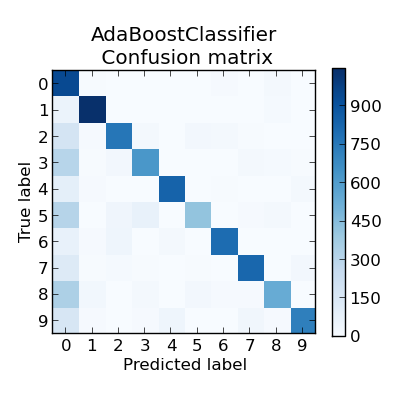
\includegraphics[width=.8\linewidth]{img/AdaBoostClassifier.png}
  %\caption{}
  %\label{fig:}
\end{minipage}%
\begin{minipage}{.5\textwidth}
  \centering
  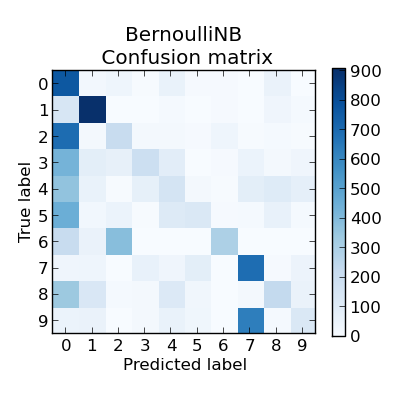
\includegraphics[width=.8\linewidth]{img/BernoulliNB.png}
  %\caption{}
  %\label{fig:} 
\end{minipage}
\begin{minipage}{.5\textwidth}
  \centering
  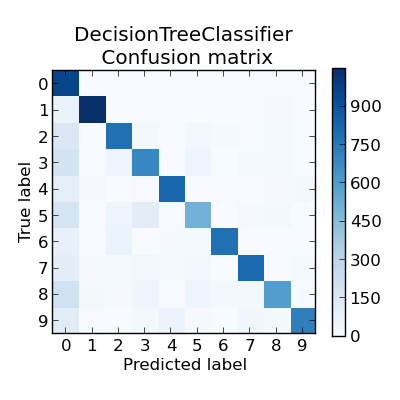
\includegraphics[width=.8\linewidth]{img/DecisionTreeClassifier.png}
  %\caption{}
  %\label{fig:}
\end{minipage}%
\begin{minipage}{.5\textwidth}
  \centering
  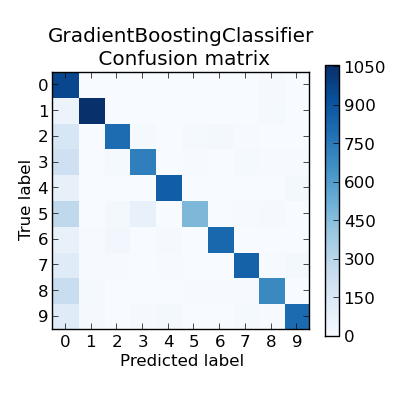
\includegraphics[width=.8\linewidth]{img/GradientBoostingClassifier.png}
  %\caption{}
  %\label{fig:} 
\end{minipage}
\begin{minipage}{.5\textwidth}
  \centering
  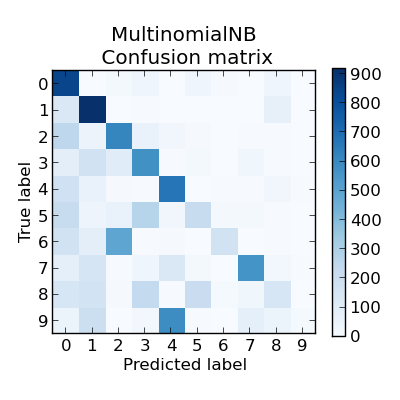
\includegraphics[width=.8\linewidth]{img/MultinomialNB.png}
  %\caption{}
  %\label{fig:}
\end{minipage}%
\begin{minipage}{.5\textwidth}
  \centering
  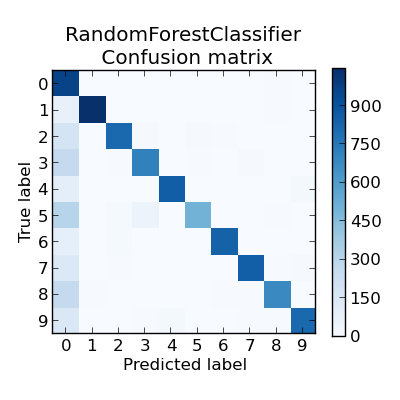
\includegraphics[width=.8\linewidth]{img/RandomForestClassifier.png}
  %\caption{}
  %\label{fig:} 
\end{minipage}
\caption{Confusion matrices.}
\label{fig:confusion}
\end{figure}

\subsubsection{ROCs}
\begin{figure}[H]
\centering
  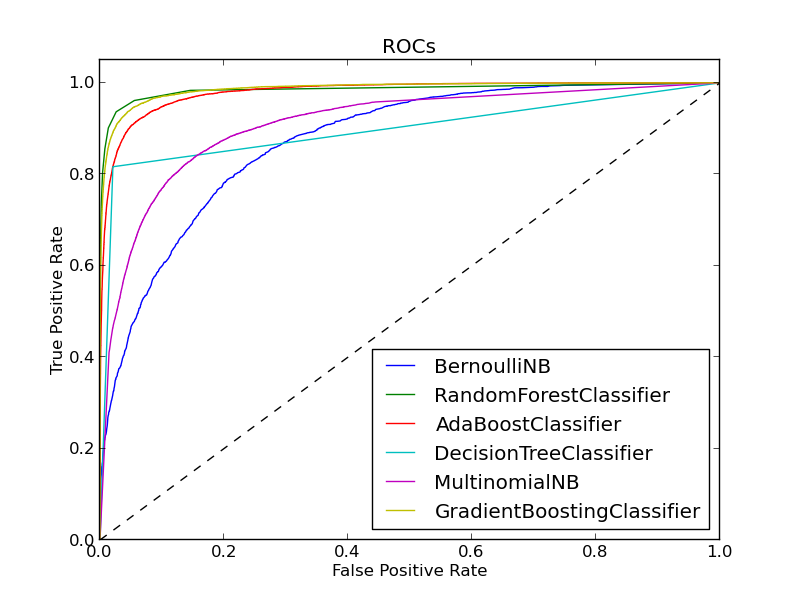
\includegraphics[width=.8\linewidth]{img/all_roc.png}
\caption{ROC curves for all classifiers.}
\label{fig:roc}
\end{figure}

As one can see from the images and also from the numbers, all classifiers had problems classifying zeros. But the RandomForestClassifier was the most successful in general, closely followed by the GradientBoostingClassifier and the AdaBoostClassifier.

The total numbers of the confusion matrix are given in table \ref{tab:confusion}. 
The single success indicators are given in table \ref{tab:dtree}.

\begin{table}[H]
\center
\begin{tabular}{c | llllllllll }
 class   &   0 &   1 &   2 &   3 &   4 &   5 &   6 &   7 &   8 & 9\\
 \hline
       0 & 965 &   2 &   0 &   0 &   0 &   1 &   3 &   1 &   8 &   0\\
       1 &  79 &1045 &   2 &   0 &   0 &   0 &   3 &   0 &   6 &   0\\
       2 & 187 &   0 & 814 &  10 &   0 &  10 &   6 &   3 &   2 &   0\\
       3 & 264 &   0 &   8 & 715 &   0 &   7 &   0 &  10 &   2 &   4\\
       4 &  98 &   0 &   1 &   0 & 859 &   0 &   0 &   3 &   1 &  20\\
       5 & 308 &   1 &  14 &  59 &   0 & 500 &   0 &   3 &   5 &   2\\
       6 &  93 &   2 &  16 &   0 &   3 &   1 & 842 &   0 &   1 &   0\\
       7 & 146 &   3 &   6 &   3 &   0 &   0 &   0 & 854 &   7 &   9\\
       8 & 263 &   6 &   0 &   3 &   0 &   4 &   7 &   5 & 685 &   1\\
       9 & 152 &   4 &   0 &   7 &  18 &   1 &   0 &   6 &   5 & 816\\
 
\end{tabular}
\caption{Confusion matrix for all classes of the DecisionTreeClassifier.}
\label{tab:confusion}
\end {table}

\begin{table}[H]
\center
\begin{tabular}{c | llll}
           class &  precision   & recall   & f1-score   & support\\
            \hline
          0  &     0.38   &   0.98    &  0.55     &  980\\
          1  &     0.98   &   0.92    &  0.95     & 1135\\
          2  &     0.95   &   0.79    &  0.86     & 1032\\
          3  &     0.90   &   0.71    &  0.79     & 1010\\
          4  &     0.98   &   0.87    &  0.92     &  982\\
          5  &     0.95   &   0.56    &  0.71     &  892\\
          6  &     0.98   &   0.88    &  0.93     &  958\\
          7  &     0.96   &   0.83    &  0.89     & 1028\\
          8  &     0.95   &   0.70    &  0.81     &  974\\
          9  &     0.96   &   0.81    &  0.88     & 1009\\
          \hline
avg / total  &     0.90   &   0.81    &  0.83     & 10000\\
\end{tabular}
\caption{Precision, recall, f1-score and support for all classes of the DecisionTreeClassifier.}
\label{tab:dtree}
\end {table}




\section{Appendix}
\subsection{Output}
The output as generated from the code given in section \ref{sec:code}.
See also classifiers.out
\lstinputlisting{classifiers.out}

\subsection{Code}
\label{sec:code}
For the code see also digitdetectorroc.py.
\lstinputlisting{digitdetectorroc.py}


%BIBLIOGRPAHY!
\bibliographystyle{plain}%amsalpha
\bibliography{bib.bib}
%\bibentry{}


%COPY AND PASTE FROM HERE

%\begin{enumerate}
% \item
%\end{enumerate}

%\href{link}{text}

%\begin[Language=Python]{lstlisting}
%#PYTHON CODE HERE
%\end{lstlisting}

%\lstinputlisting[language=Java]{ }

%\csvautotabular[separator=semicolon]{data.csv}

%\begin{figure}
% \center
% \includegraphics[width= cm]{img/ }
% \caption{}
%\end{figure}



\end{document}
